\documentclass[11pt,a4paper]{article}

\usepackage[margin=1in]{geometry}
\usepackage[T1]{fontenc}
\usepackage[utf8]{inputenc}
\IfFileExists{lmodern.sty}{\usepackage{lmodern}}{}
\usepackage[expansion=false]{microtype}
\usepackage{amsmath,amssymb,amsthm,mathtools}
\usepackage{booktabs}
\usepackage{array}
\usepackage{graphicx}
\usepackage{enumitem}
\usepackage{xcolor}
\usepackage{hyperref}
\usepackage{pgfplots}
\pgfplotsset{compat=1.18}

\hypersetup{
  colorlinks=true,
  linkcolor=blue!50!black,
  citecolor=blue!50!black,
  urlcolor=blue!50!black,
  pdftitle={A Phase Law for Mixed-Base Tetration},
  pdfauthor={Janis Justus}
}

\theoremstyle{plain}
\newtheorem{theorem}{Theorem}[section]
\newtheorem{proposition}[theorem]{Proposition}
\newtheorem{lemma}[theorem]{Lemma}
\newtheorem{corollary}[theorem]{Corollary}
\newtheorem{conjecture}[theorem]{Conjecture}

\theoremstyle{definition}
\newtheorem{definition}[theorem]{Definition}
\newtheorem{hypothesis}[theorem]{Hypothesis}

\theoremstyle{remark}
\newtheorem{remark}[theorem]{Remark}

\newcommand{\R}{\mathbb{R}}
\newcommand{\N}{\mathbb{N}}
\newcommand{\dd}{\,\mathrm{d}}
\newcommand{\slog}{\operatorname{slog}}
\newcommand{\Log}{\operatorname{Log}}
\newcommand{\id}{\operatorname{id}}
\newcommand{\norm}[1]{\left\lVert #1\right\rVert}
\newcommand{\abs}[1]{\left\lvert #1\right\rvert}
\newcommand{\set}[1]{\left\{#1\right\}}
\newcommand{\floor}[1]{\left\lfloor #1\right\rfloor}
\newcommand{\bbd}{b,d}

\title{A Phase Law for Mixed-Base Tetration:\\Logarithmic Tails, Cocycle Structure, and Singular Asymptotics}
\author{Janis Justus}
\date{June 2026}

\begin{document}
\maketitle

\begin{abstract}
We study the mixed-base height map
\[
  F_{b,d}(x):=\slog_b(T_d(x)),
\]
where $T_d$ and $T_b$ are regular tetration branches and $\slog_b=T_b^{-1}$ is the corresponding Abel coordinate for the outer base $b$.  The paper is formulated for the Paulsen--Cowgill/Kneser regular tetration branches, in particular for real bases above the classical threshold $e^{1/e}$, while making explicit the additional real-channel estimates used in the proof.  Along integer heights, exact Abel peeling produces diagonal logarithmic constants and hence a constant asymptotic shift.  For real heights, however, numerical phase profiles for $b,d\in\{2,e,10\}$ show that $F_{b,d}(x)-x$ is not asymptotically scalar; it approaches a small periodic function of the fractional height.

The main theorem proves a conditional phase law.  Under a regular real-logarithmic channel and a uniform peeling-growth estimate, the logarithmic tails
\[
  D_n^{b,d}(\theta)=L_b^{\circ n}(T_d(n+\theta))
\]
converge uniformly on the phase circle.  Consequently
\[
  \slog_b(T_d(x))-x=\mu_{b,d}+P_{b,d}(\{x\})+o(1),\qquad x\to+\infty,
\]
with $P_{b,d}$ centered and $1$-periodic.  We also prove the exact groupoid identity $F_{b,d}=F_{b,c}\circ F_{c,d}$, derive the associated nonlinear phase cocycle, prove exact inverse mean antisymmetry under a smooth circle-diffeomorphism assumption, and record the logarithmic singular expansion of real tetration near $x=-2$.  The results separate exact algebraic identities, conditional analytic theorems for the regular branch, and numerical phenomena such as Fourier dominance and the approximate rank-one inner-base law.
\end{abstract}


\section{Introduction}

Regular tetration to a base $b$ is a function $T_b$ satisfying
\begin{equation}\label{eq:tetration}
  T_b(0)=1,\qquad T_b(x+1)=b^{T_b(x)}.
\end{equation}
For real bases $b>e^{1/e}$ we use the regular branch constructed in the Kneser--Paulsen tradition: Kneser's construction gives the classical holomorphic tetration for the natural base, while Paulsen and Cowgill give conditions determining a unique solution of $F(z+1)=b^{F(z)}$ for real $b>e^{1/e}$; Paulsen later extends the framework to complex bases \cite{kneser1950,kouznetsov2009,paulsen-cowgill,paulsen-complex-bases}.  The inverse of $T_b$, where defined, is the superlogarithm
\[
  A_b:=T_b^{-1}=\slog_b.
\]
This paper studies the following mixed-base problem: what happens when a tower generated with one base is measured in the height coordinate of another base?  The object that records this conversion is
\begin{equation}\label{eq:Fbd}
  F_{b,d}(x):=A_b(T_d(x))=\slog_b(T_d(x)).
\end{equation}
A natural first expectation is that $F_{b,d}$ should be asymptotically a translation,
\[
  F_{b,d}(x)\approx x+\text{constant}.
\]
This is exactly what integer heights suggest.  However, real heights contain an additional phase variable.  Numerical experiments with $b,d\in\{2,e,10\}$ indicate that the residual
\[
  F_{b,d}(x)-x
\]
does not converge to one scalar value.  Instead, it settles into a small $1$-periodic profile depending on the fractional part $\{x\}$.

The structural form suggested by the data is
\begin{equation}\label{eq:intro-phase}
  F_{b,d}(x)-x=\mu_{b,d}+P_{b,d}(\{x\})+o(1),\qquad x\to+\infty,
\end{equation}
where $\mu_{b,d}$ is a mean shift and $P_{b,d}$ is a centered periodic correction.  The purpose of the paper is to explain why such a phase should exist and how it is organized.

The mechanism is logarithmic peeling.  Let
\[
  L_b(y):=\log_b(y)=\frac{\log y}{\log b}.
\]
The Abel identity
\begin{equation}\label{eq:abel}
  A_b(b^y)=A_b(y)+1
\end{equation}
is equivalently
\begin{equation}\label{eq:abel-log}
  A_b(y)=1+A_b(L_b(y))
\end{equation}
whenever the logarithm lies on the chosen branch.  Thus each application of $L_b$ removes one unit of $b$-height.  For $x=n+\theta$ with $0\leq\theta<1$, define
\begin{equation}\label{eq:Dndef-intro}
  D_n^{b,d}(\theta):=L_b^{\circ n}(T_d(n+\theta)).
\end{equation}
Then exact Abel peeling gives
\begin{equation}\label{eq:peeling-intro}
  F_{b,d}(n+\theta)-(n+\theta)=A_b(D_n^{b,d}(\theta))-\theta.
\end{equation}
The phase law is therefore reduced to the convergence of the functions $D_n^{b,d}(\theta)$, uniformly in the phase variable $\theta$.

The new proof ingredient is that the transition from height $n$ to height $n+1$ introduces only the fixed base-mismatch factor
\begin{equation}\label{eq:alpha-intro}
  \alpha=\log_b d.
\end{equation}
Indeed,
\[
  T_d(n+1+\theta)=d^{T_d(n+\theta)}
\]
and hence
\[
  L_b(T_d(n+1+\theta))=\alpha T_d(n+\theta).
\]
Thus $D_{n+1}^{b,d}$ and $D_n^{b,d}$ differ by applying $n$ logarithms to $\alpha Y$ and $Y$.  The first logarithm turns this multiplicative discrepancy into an additive constant.  Each further logarithm divides the remaining error by the current tower level.  Under a regular real-channel assumption and a uniform peeling-growth estimate, the resulting damping products are summable, and the logarithmic tails converge uniformly.

The contribution of the paper is fourfold.  First, it gives exact integer and real-height peeling identities.  Second, it proves a conditional phase theorem for the regular real branch by logarithmic-tail convergence.  Third, it shows that the mixed-base height maps form an exact groupoid, yielding a nonlinear cocycle law for the limiting phases.  Fourth, it records a singular expansion near $x=-2$, showing that the same functional equation also imposes rigid behavior at the left boundary of the real branch.

The word ``conditional'' is important.  The tetration branch itself is not arbitrary: the intended branch is the Paulsen--Cowgill/Kneser regular tetration branch.  The remaining analytic difficulty is to derive the real-channel and uniform peeling-growth estimates directly from that construction.  Until that is done, the phase theorem should be read as a precise reduction of the phase law to explicit analytic estimates on the regular branch, supported by numerical evidence.

\section{Preliminaries and branch assumptions}


\subsection{The regular branch used in this paper}

For each admissible base $a$ we write $T_a$ for the regular tetration branch satisfying \eqref{eq:tetration}, and $A_a=T_a^{-1}$ for its Abel inverse.  In the real numerical work and in the intended application of the phase theorem, $a$ is a real base with $a>e^{1/e}$ and $T_a$ is the Paulsen--Cowgill regular tetration branch.  This choice is essential: without a complex or global regularity condition, real-analytic solutions of the tetration equation are not unique.  The uniqueness theory for holomorphic Abel functions and regular tetration is the background that makes the mixed-base comparison meaningful \cite{paulsen-cowgill,trappmann-kouznetsov}.

The Abel equation is \eqref{eq:abel}, and the logarithmic peeling form is \eqref{eq:abel-log}.  Throughout, $L_b^{\circ n}$ means the $n$-fold iterate of $L_b$.  The notation is chosen so that $b$ is always the outer base, i.e. the base of the logarithmic peeling and of the superlogarithm, while $d$ is the inner base generating the tower.

\begin{definition}[Mixed-base height map]
For two admissible bases $b,d$, define
\[
  F_{b,d}:=A_b\circ T_d,\qquad F_{b,d}(x)=\slog_b(T_d(x)).
\]
Thus $F_{b,d}$ converts height in the $d$-tetration coordinate to height in the $b$-tetration coordinate.
\end{definition}

\subsection{A regular real-logarithmic channel}

The repeated logarithms used below must stay on a coherent real branch.  We isolate this as an assumption.

\begin{hypothesis}[Regular real-logarithmic channel]\label{hyp:channel}
For the pair $(T_b,T_d)$ we assume:
\begin{enumerate}[label=(R\arabic*),leftmargin=2em]
  \item $T_d$ is positive and continuous on $[0,\infty)$, and on each compact interval $[r,r+1]$ its values are bounded above and below away from zero.
  \item For all sufficiently large $n$ and every $\theta\in[0,1]$, the logarithmic iterates $L_b^{\circ k}(T_d(n+\theta))$ used below remain in the chosen real logarithmic channel until the final value lies in a fixed compact subset of the real domain of $A_b$.
  \item The branch $A_b$ is continuous and locally Lipschitz on a compact neighborhood containing all limiting logarithmic tails considered below.
\end{enumerate}
\end{hypothesis}

\begin{remark}
For the Paulsen--Cowgill branch above the real fixed-point threshold $e^{1/e}$, these assumptions express the real logarithmic reduction process used in computation.  The point of the main theorem is to show that once these channel estimates are available, the phase law follows by a contraction argument.
\end{remark}

\subsection{Uniform peeling growth}

The original proof sketch used the estimate
\[
  L_b^{\circ k}(T_d(n+\theta))\geq c_m T_d(n-k+\theta)-B_m
\]
and then concluded summability of a product of reciprocal tower levels.  This is the correct idea, but to make the proof clean one must control the estimate uniformly in $n,k$ and $\theta$.  We therefore state the needed uniform growth explicitly.

\begin{hypothesis}[Uniform peeling growth]\label{hyp:peeling-growth}
There exist constants $M\in\N$, $a>0$, and $B\geq0$ such that for all sufficiently large $n$, all $\theta\in[0,1]$, and all $1\leq k\leq n-M$,
\begin{equation}\label{eq:uniform-peeling-growth}
  L_b^{\circ k}(T_d(n+\theta))\geq a\,T_d(n-k+\theta)-B.
\end{equation}
Moreover, if
\begin{equation}\label{eq:sj-def}
  s_j:=\inf_{0\leq\theta\leq1}T_d(j+\theta),
\end{equation}
then $s_j\to+\infty$.
\end{hypothesis}

\begin{remark}[Why this is the right strengthening]\label{rem:threshold}
The condition $s_j\to+\infty$ is automatic for strongly growing real towers.  In particular, it is natural for bases $d>e^{1/e}$ on the regular increasing real branch.  It is not automatic for all $d>1$: below or at the real fixed-point threshold, the forward iteration of $x\mapsto d^x$ can remain bounded.  Therefore a theorem stated merely for all $b,d>1$ would be too broad unless the channel and growth assumptions are replaced by something else.
\end{remark}

\begin{remark}[Status of the hypotheses]\label{rem:hyp-status}
Both hypotheses have since been discharged for the intended branch class.
First, $s_j\to\infty$ is \emph{automatic} for every $d>e^{1/e}$, with the
explicit gap $d^{\,x}-x\ge(1+\ln\ln d)/\ln d>0$ (Lemma~\ref{lem:D-growth} in
Appendix~\ref{app:stopped}).  Second, positivity of the logarithmic chain --
the content of (R2) in Hypothesis~\ref{hyp:channel} -- holds
\emph{unconditionally} for the chain stopped at an explicit level
$J_0=\min\{j:\ T_d(j)\ge 2C_0\}$, by a self-contained downward induction
(the \emph{Stoppregel}, Lemma~\ref{lem:D-stop}); and for the limit objects
the correct channel statement is offset-aligned
(Lemma~\ref{lem:D-offset}), which in particular covers skew pairs such as
$(b,d)=(10,2)$ with $\mu_{10,2}<-2$, where the unshifted reading fails.
All estimates of the present paper apply verbatim to the stopped chain; see
Appendix~\ref{app:stopped} and the companion notes
\cite{justus-diffeo-note,justus-stoppregel-note}.
\end{remark}

\section{Integer basis change and diagonal logarithmic constants}

The integer theory is the simplest part of the story.  It is exact and explains why one initially expects a constant shift.

\begin{definition}[Diagonal logarithmic tails]
For integer $n\geq0$, define
\begin{equation}\label{eq:Cn-def}
  C_n^{b,d}:=L_b^{\circ n}(T_d(n)),
\end{equation}
whenever the $n$-fold logarithm is defined.
\end{definition}

\begin{proposition}[Exact integer peeling]\label{prop:integer-peeling}
For every integer $n$ for which the iterated logarithms are defined,
\begin{equation}\label{eq:integer-peeling}
  A_b(T_d(n))=n+A_b(C_n^{b,d}).
\end{equation}
Equivalently,
\[
  \slog_b(T_d(n))=n+\slog_b(C_n^{b,d}).
\]
\end{proposition}

\begin{proof}
Iterating \eqref{eq:abel-log} exactly $n$ times gives
\[
  A_b(y)=n+A_b(L_b^{\circ n}(y)).
\]
Now substitute $y=T_d(n)$.
\end{proof}

\begin{corollary}[Integer basis-change law]\label{cor:integer-law}
Assume that $C_n^{b,d}\to C_{b,d}$ and that $A_b$ is continuous at $C_{b,d}$.  Then
\begin{equation}\label{eq:integer-law}
  \slog_b(T_d(n))=n+\slog_b(C_{b,d})+o(1),\qquad n\to\infty.
\end{equation}
Equivalently,
\[
  T_d(n)=T_b\bigl(n+\slog_b(C_{b,d})+o(1)\bigr).
\]
\end{corollary}

\begin{remark}[Integer heights see only one phase]
The constant $\slog_b(C_{b,d})$ is not the mean shift of the real-height phase profile.  It is the value of the phase at $\theta=0$.  This distinction becomes important later.
\end{remark}

\subsection{First correction at integer heights}

The exact identity also gives a correction term by Taylor expansion.

\begin{proposition}[First correction]\label{prop:first-correction}
Assume $C_n^{b,d}\to C_{b,d}$ and $A_b$ is $C^2$ near $C_{b,d}$.  Then
\begin{equation}\label{eq:first-correction}
  \slog_b(T_d(n))=n+\slog_b(C_{b,d})+A_b'(C_{b,d})(C_n^{b,d}-C_{b,d})+O((C_n^{b,d}-C_{b,d})^2).
\end{equation}
\end{proposition}

\begin{proof}
From Proposition \ref{prop:integer-peeling}, $A_b(T_d(n))=n+A_b(C_n^{b,d})$.  Taylor expand $A_b(C_n^{b,d})$ around $C_{b,d}$.
\end{proof}

For $b=e$, the same damping mechanism predicts hyper-exponentially fast convergence of $C_n^{e,d}$ to its limiting constant: each additional logarithmic peel multiplies the remaining error by approximately the reciprocal of the current tower level.

\section{Numerical evidence for real-height phase profiles}

The integer law does not describe real heights.  The relevant residual is
\begin{equation}\label{eq:raw-residual}
  \widetilde P_{b,d}(x):=F_{b,d}(x)-x=\slog_b(T_d(x))-x.
\end{equation}
Numerically, for $b,d\in\{2,e,10\}$, $b\ne d$, this residual does not settle to a scalar constant.  It is much better described by
\begin{equation}\label{eq:numeric-phase-model}
  \widetilde P_{b,d}(x)=\mu_{b,d}+P_{b,d}(\{x\})+o(1).
\end{equation}

For a large reference height, such as $x=6+\theta$, the centered phase profile is computed as
\begin{equation}\label{eq:centered-profile}
  P_{b,d}(\theta)=\slog_b(T_d(6+\theta))-(6+\theta)-\mu_{b,d},\qquad 0\leq\theta<1,
\end{equation}
where $\mu_{b,d}$ is the period average.  Its real Fourier expansion is
\begin{equation}\label{eq:fourier-real}
  P_{b,d}(\theta)\sim\sum_{k\geq1}\left(a_k\cos(2\pi k\theta)+b_k\sin(2\pi k\theta)\right).
\end{equation}

\begin{table}[htbp]
\centering
\caption{Numerical mean shifts and first-harmonic data for the six ordered pairs from $\{2,e,10\}$.  The centered profile is fitted as $P_{b,d}(\theta)\approx A_1\sin(2\pi\theta+\phi_{b,d})$.}
\resizebox{\textwidth}{!}{%
\begin{tabular}{@{}ccccccc@{}}
\toprule
$(b,d)$ & $\mu_{b,d}$ & $A_1$ & $\phi_{b,d}$ & $A_2/A_1$ & RMS$_1$ & RMS$_3$ \\
\midrule
$(e,2)$   & $-1.12840377662892400988$ & $1.436658218\cdot10^{-4}$ & $0.5144443757$ & $0.0095584109$ & $9.71405\cdot10^{-7}$ & $1.29711\cdot10^{-9}$ \\
$(2,e)$   & $+1.12840377662892400988$ & $1.436663862\cdot10^{-4}$ & $4.4628232922$ & $0.0091384299$ & $9.28728\cdot10^{-7}$ & $1.26823\cdot10^{-9}$ \\
$(2,10)$  & $+2.26496083873884752865$ & $4.607972095\cdot10^{-4}$ & $5.3516038121$ & $0.0086504936$ & $2.81980\cdot10^{-6}$ & $4.02796\cdot10^{-9}$ \\
$(e,10)$  & $+1.13655705571332644090$ & $3.172285062\cdot10^{-4}$ & $5.3655348200$ & $0.0088511875$ & $1.98628\cdot10^{-6}$ & $2.81454\cdot10^{-9}$ \\
$(10,e)$  & $-1.13655705571332644090$ & $3.172256724\cdot10^{-4}$ & $1.3659262980$ & $0.0098080450$ & $2.20097\cdot10^{-6}$ & $2.94538\cdot10^{-9}$ \\
$(10,2)$  & $-2.26496083873884752865$ & $4.607912773\cdot10^{-4}$ & $0.5452089842$ & $0.0100280230$ & $3.26875\cdot10^{-6}$ & $4.31141\cdot10^{-9}$ \\
\bottomrule
\end{tabular}}
\label{tab:phase-summary}
\end{table}

Several features stand out.  First, the second harmonic is below about $1.1\%$ of the first in all six cases.  Second, adding only a few harmonics improves the residual error dramatically.  Third, the mean shifts are antisymmetric to working precision: in the July~2026 recomputation with the stopped exact peeling of Appendix~\ref{app:stopped} (256--2048 samples, 80--260 digits),
\[
  |\mu_{b,d}+\mu_{d,b}|\ \le\ 10^{-38}
\]
for all six ordered pairs.  The residuals of order $10^{-8}$--$10^{-11}$ reported in an earlier version of this table were finite-height and quadrature artifacts of the original pipeline; by Theorem~B of the companion note \cite{justus-diffeo-note} the antisymmetry is exactly zero in the limit, unconditionally.  (The table above lists the recomputed values; $\mu$ is stated to twenty digits and is available to $180$ digits for $(e,2)$.)

\begin{figure}[htbp]
\centering
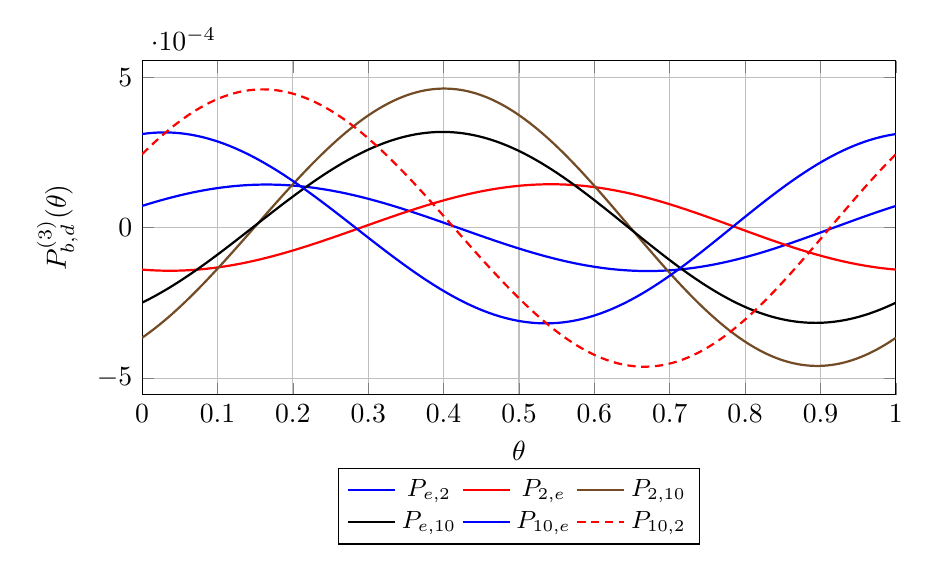
\begin{tikzpicture}
\begin{axis}[
  width=0.92\textwidth,
  height=0.48\textwidth,
  xlabel={$\theta$},
  ylabel={$P_{b,d}^{(3)}(\theta)$},
  xmin=0,xmax=1,
  grid=both,
  legend columns=3,
  legend style={font=\small,at={(0.5,-0.22)},anchor=north},
  samples=200,
  domain=0:1
]
\addplot+[mark=none,thick] {7.0709128210e-5*cos(deg(2*pi*x)) + 1.2507369316e-4*sin(deg(2*pi*x)) + 1.3686522925e-6*cos(deg(4*pi*x)) + 2.4721384890e-7*sin(deg(4*pi*x)) + 5.3885273349e-8*cos(deg(6*pi*x)) + 1.0471715325e-8*sin(deg(6*pi*x))};
\addlegendentry{$P_{e,2}$}
\addplot+[mark=none,thick] {-1.3921565139e-4*cos(deg(2*pi*x)) - 3.5483182068e-5*sin(deg(2*pi*x)) - 1.5249634216e-7*cos(deg(4*pi*x)) + 1.3039910022e-6*sin(deg(4*pi*x)) + 2.5710726750e-8*cos(deg(6*pi*x)) + 2.7099947223e-8*sin(deg(6*pi*x))};
\addlegendentry{$P_{2,e}$}
\addplot+[mark=none,thick] {-3.6981944012e-4*cos(deg(2*pi*x)) + 2.7489570700e-4*sin(deg(2*pi*x)) + 3.9823572422e-6*cos(deg(4*pi*x)) - 1.7322902236e-7*sin(deg(4*pi*x)) - 1.7515598225e-8*cos(deg(6*pi*x)) - 1.1398397289e-7*sin(deg(6*pi*x))};
\addlegendentry{$P_{2,10}$}
\addplot+[mark=none,thick] {-2.5193527971e-4*cos(deg(2*pi*x)) + 1.9277587935e-4*sin(deg(2*pi*x)) + 2.8063483939e-6*cos(deg(4*pi*x)) - 9.1791060602e-8*sin(deg(4*pi*x)) - 1.2741476598e-8*cos(deg(6*pi*x)) - 8.0227555110e-8*sin(deg(6*pi*x))};
\addlegendentry{$P_{e,10}$}
\addplot+[mark=none,thick] {3.1059185436e-4*cos(deg(2*pi*x)) + 6.4536380289e-5*sin(deg(2*pi*x)) + 4.4133415828e-7*cos(deg(4*pi*x)) - 3.0798912056e-6*sin(deg(4*pi*x)) - 6.2066334690e-8*cos(deg(6*pi*x)) - 6.3625884293e-8*sin(deg(6*pi*x))};
\addlegendentry{$P_{10,e}$}
\addplot+[mark=none,thick] {2.3902453213e-4*cos(deg(2*pi*x)) + 3.9399535840e-4*sin(deg(2*pi*x)) + 4.5910531565e-6*cos(deg(4*pi*x)) + 9.0102205891e-7*sin(deg(4*pi*x)) + 1.8061346343e-7*cos(deg(6*pi*x)) + 3.3438721149e-8*sin(deg(6*pi*x))};
\addlegendentry{$P_{10,2}$}
\end{axis}
\end{tikzpicture}
\caption{Three-mode Fourier reconstruction of the six centered phase profiles from the numerical data.  The near-sinusoidal shape reflects the dominance of the first Fourier mode.}
\label{fig:phase-profiles}
\end{figure}

These data motivate two conjectures.

The inverse-pair sums are so small that they should not be interpreted merely as a weak numerical accident.  Section \ref{sec:cocycle} shows that, once the limiting phase maps are smooth circle diffeomorphisms, inverse mean antisymmetry follows exactly.

\begin{conjecture}[Rank-one inner-base phase law]\label{conj:inner-base}
For each fixed inner base $d$, the family of centered phase profiles
\[
  \{P_{b,d}: b\neq d\}
\]
is approximately rank one in $L^2(S^1)$.  Equivalently, after normalization by $L^2$ norm and a possible sign, the shape of $P_{b,d}$ depends primarily on the inner base $d$, while the outer base mainly changes the amplitude and phase shift.
\end{conjecture}

\begin{remark}[Quantified status of Conjecture~\ref{conj:inner-base}]
The rank-one law is now understood as the leading order of a linear-response
expansion in the gauge parameter $\beta=\ln\ln b$: writing
$\varepsilon=\ln\ln b-\ln\ln d$, one has
$\widehat P_{b,d}(k)=\varepsilon\,\widehat G_k(d)+\varepsilon^2\widehat
H_k(d)+O(\varepsilon^3)$, where $G_d=\partial_\beta\Phi_{b,d}|_{b=d}$ is the
response kernel of the inner base.  The kernels $G_d$ (and the second-order
kernels $H_d$) have been computed to $25$--$30$ digits for
$d\in\{2,e,3,5,10\}$ by two independent routes (complex-step differentiation
of the regular branch through base holomorphy \cite{paulsen-complex-bases},
and $\varepsilon$-stencils of the base family); the expansion reproduces all
measured pairs with third-order-small residuals up to $|\varepsilon|=1.2$.
The measured deviation from exact rank one is a smooth $d$-dependence of the
normalized mode ratios $|G_k|/|G_1|$ of about $0.4\%$ at $k=2$, growing to
$\approx9\%$ at $k=8$.
\end{remark}

\section{Logarithmic-tail convergence}

We now prove the conditional phase theorem.  The proof starts with exact peeling and then turns the convergence problem into an error-damping estimate.

\subsection{Exact real-height peeling}

For $x=n+\theta$, $n\in\N$, $0\leq\theta<1$, define
\begin{equation}\label{eq:Dn-def}
  D_n(\theta):=D_n^{b,d}(\theta):=L_b^{\circ n}(T_d(n+\theta)).
\end{equation}

\begin{proposition}[Exact phase peeling]\label{prop:exact-phase-peeling}
For every $n$ for which the iterated logarithms are defined,
\begin{equation}\label{eq:exact-phase-peeling}
  \slog_b(T_d(n+\theta))-(n+\theta)=A_b(D_n(\theta))-\theta.
\end{equation}
\end{proposition}

\begin{proof}
Iterating \eqref{eq:abel-log} exactly $n$ times gives
\[
  A_b(y)=n+A_b(L_b^{\circ n}(y)).
\]
Substitute $y=T_d(n+\theta)$.  Then
\[
  A_b(T_d(n+\theta))=n+A_b(L_b^{\circ n}(T_d(n+\theta)))=n+A_b(D_n(\theta)).
\]
Subtracting $n+\theta$ gives \eqref{eq:exact-phase-peeling}.
\end{proof}

Thus the entire phase law reduces to proving that $D_n(\theta)$ converges uniformly in $\theta$.

\subsection{The base mismatch}

Set
\begin{equation}\label{eq:alpha}
  \alpha:=\log_b d=\frac{\log d}{\log b}>0.
\end{equation}
The only mismatch between the $d$-tower and the $b$-logarithmic peeling is this factor.  Indeed,
\[
  T_d(n+1+\theta)=d^{T_d(n+\theta)},
\]
so
\begin{align}
  D_{n+1}(\theta)
  &=L_b^{\circ(n+1)}(T_d(n+1+\theta))\notag\\
  &=L_b^{\circ n}(L_b(d^{T_d(n+\theta)}))\notag\\
  &=L_b^{\circ n}(\alpha T_d(n+\theta)).\label{eq:Dnplus-alpha}
\end{align}
On the other hand,
\[
  D_n(\theta)=L_b^{\circ n}(T_d(n+\theta)).
\]
Therefore, with $Y_n(\theta):=T_d(n+\theta)$,
\begin{equation}\label{eq:dn-diff-alpha}
  D_{n+1}(\theta)-D_n(\theta)=L_b^{\circ n}(\alpha Y_n(\theta))-L_b^{\circ n}(Y_n(\theta)).
\end{equation}
The task is to show that an initial fixed multiplicative difference $Y\mapsto\alpha Y$ is killed by $n$ logarithms.

\begin{lemma}[One-step damping]\label{lem:one-step}
Let $u>0$, $v>0$, and suppose $\abs{v-u}\leq u/2$.  Then
\begin{equation}\label{eq:one-step-damping}
  \abs{L_b(v)-L_b(u)}\leq \frac{2}{\log b}\frac{\abs{v-u}}{u}.
\end{equation}
\end{lemma}

\begin{proof}
Write $v=u+\delta$ with $\abs{\delta}\leq u/2$.  Then
\[
  L_b(v)-L_b(u)=\frac{1}{\log b}\log\left(1+\frac{\delta}{u}\right).
\]
For $\abs{t}\leq1/2$, $\abs{\log(1+t)}\leq2\abs{t}$.  This gives the result.
\end{proof}

\begin{lemma}[Iterated damping product]\label{lem:iterated-damping}
Fix a cutoff $m\geq1$.  Under Hypothesis \ref{hyp:channel}, there are constants $C_m>0$ and $N_m$ such that for all $n\geq N_m$ and all $\theta\in[0,1]$,
\begin{equation}\label{eq:iterated-damping}
  \abs{D_{n+1}(\theta)-D_n(\theta)}
  \leq C_m\prod_{k=1}^{n-m}\frac{1}{L_b^{\circ k}(T_d(n+\theta))}.
\end{equation}
\end{lemma}

\begin{proof}
Let
\[
  U_0:=T_d(n+\theta),\qquad V_0:=\alpha T_d(n+\theta),
\]
and define recursively
\[
  U_{k+1}:=L_b(U_k),\qquad V_{k+1}:=L_b(V_k).
\]
Then $U_n=D_n(\theta)$ and $V_n=D_{n+1}(\theta)$.  Put $\delta_k:=V_k-U_k$.  The first logarithm gives the exact identity
\[
  \delta_1=L_b(\alpha U_0)-L_b(U_0)=L_b(\alpha),
\]
which is independent of $U_0$.

For $k\geq1$,
\[
  \delta_{k+1}=L_b(U_k+\delta_k)-L_b(U_k).
\]
On the first $n-m$ iterates the real-channel and growth assumptions ensure, after increasing $N_m$ if necessary, that $U_k$ is uniformly large and $\abs{\delta_k}\leq U_k/2$.  Applying Lemma \ref{lem:one-step} inductively yields
\[
  \abs{\delta_{n-m}}
  \leq C\prod_{k=1}^{n-m}\frac{1}{U_k}
  =C\prod_{k=1}^{n-m}\frac{1}{L_b^{\circ k}(T_d(n+\theta))}.
\]
The remaining $m$ logarithms take place in the fixed compact real channel from Hypothesis \ref{hyp:channel}; there $L_b^{\circ m}$ is Lipschitz.  Absorbing its Lipschitz constant into $C_m$ gives \eqref{eq:iterated-damping}.
\end{proof}

\subsection{The improved summability argument}

The next lemma is the cleaned-up version of the critical step.  Instead of relying on an informal tower-height statement, it uses Hypothesis \ref{hyp:peeling-growth} explicitly.

\begin{lemma}[Summability of the damping products]\label{lem:summability}
Assume Hypotheses \ref{hyp:channel} and \ref{hyp:peeling-growth}.  Then there is $N$ such that
\begin{equation}\label{eq:summability}
  \sum_{n=N}^{\infty}\sup_{0\leq\theta\leq1}\abs{D_{n+1}(\theta)-D_n(\theta)}<\infty.
\end{equation}
\end{lemma}

\begin{proof}
By Lemma \ref{lem:iterated-damping}, for fixed $m\geq M$,
\[
  \abs{D_{n+1}(\theta)-D_n(\theta)}
  \leq C_m\prod_{k=1}^{n-m}\frac{1}{L_b^{\circ k}(T_d(n+\theta))}.
\]
Using \eqref{eq:uniform-peeling-growth}, for all sufficiently large $n$ and $1\leq k\leq n-m$,
\[
  L_b^{\circ k}(T_d(n+\theta))\geq aT_d(n-k+\theta)-B.
\]
Since $s_j\to+\infty$, after increasing $N$ we may assume $a s_j-B\geq (a/2)s_j$ for all $j\geq m$.  Hence, uniformly in $\theta$,
\[
  L_b^{\circ k}(T_d(n+\theta))\geq \frac a2\,s_{n-k}.
\]
Therefore
\[
  \abs{D_{n+1}(\theta)-D_n(\theta)}
  \leq C'_m\prod_{k=1}^{n-m}\frac{1}{s_{n-k}}
  =C'_m\prod_{j=m}^{n-1}\frac1{s_j}.
\]
Because $s_j\to+\infty$, there exists $J\geq m$ such that $s_j\geq2$ for all $j\geq J$.  Hence
\[
  \prod_{j=m}^{n-1}\frac1{s_j}\leq C''2^{-n}
\]
for all sufficiently large $n$.  The geometric series $\sum_n2^{-n}$ converges, and taking the supremum over $\theta$ gives \eqref{eq:summability}.
\end{proof}

\begin{remark}[What was repaired]
The contraction argument depends not only on the intuitive fact that logarithms reduce effective tower height one level at a time, but also on uniformity.  The error term must not grow with $n$, $k$, or $\theta$, and the supremum over all phases requires a uniform lower bound.  Hypothesis \ref{hyp:peeling-growth} and the sequence $s_j=\inf_\theta T_d(j+\theta)$ make this uniformity explicit.
\end{remark}

\subsection{Uniform convergence and the phase law}

\begin{theorem}[Mixed-base logarithmic-tail convergence]\label{thm:tail-convergence}
Under Hypotheses \ref{hyp:channel} and \ref{hyp:peeling-growth}, the functions
\[
  D_n(\theta)=L_b^{\circ n}(T_d(n+\theta))
\]
converge uniformly on $[0,1]$ to a limiting tail profile
\begin{equation}\label{eq:limit-tail}
  D_{b,d}(\theta):=\lim_{n\to\infty}D_n(\theta).
\end{equation}
\end{theorem}

\begin{proof}
By Lemma \ref{lem:summability},
\[
  \sum_{n=N}^{\infty}\norm{D_{n+1}-D_n}_\infty<\infty.
\]
Therefore $(D_n)$ is uniformly Cauchy in the sup norm on $[0,1]$.  Since the space of continuous real-valued functions on $[0,1]$ is complete, $D_n$ converges uniformly to a continuous limiting function $D_{b,d}$.
\end{proof}

\begin{theorem}[Mixed-base phase law]\label{thm:phase-law}
Under Hypotheses \ref{hyp:channel} and \ref{hyp:peeling-growth}, define
\begin{equation}\label{eq:Phi-def}
  \Phi_{b,d}(\theta):=A_b(D_{b,d}(\theta))-\theta,
  \qquad 0\leq\theta<1.
\end{equation}
Then, as $x\to+\infty$,
\begin{equation}\label{eq:phase-law}
  \slog_b(T_d(x))-x=\Phi_{b,d}(\{x\})+o(1).
\end{equation}
Equivalently,
\begin{equation}\label{eq:mean-phase-law}
  \slog_b(T_d(x))-x=\mu_{b,d}+P_{b,d}(\{x\})+o(1),
\end{equation}
where
\begin{equation}\label{eq:mean-centered-def}
  \mu_{b,d}:=\int_0^1\Phi_{b,d}(\theta)\dd\theta,
  \qquad
  P_{b,d}(\theta):=\Phi_{b,d}(\theta)-\mu_{b,d}.
\end{equation}
The function $P_{b,d}$ is $1$-periodic after periodic extension and has mean zero.
\end{theorem}

\begin{proof}
Write $x=n+\theta$ with $n=\floor{x}$ and $0\leq\theta<1$.  By Proposition \ref{prop:exact-phase-peeling},
\[
  \slog_b(T_d(x))-x=A_b(D_n(\theta))-\theta.
\]
By Theorem \ref{thm:tail-convergence}, $D_n(\theta)\to D_{b,d}(\theta)$ uniformly.  Since $A_b$ is locally Lipschitz on the relevant compact set,
\[
  A_b(D_n(\theta))-\theta=A_b(D_{b,d}(\theta))-\theta+o(1)=\Phi_{b,d}(\theta)+o(1),
\]
uniformly in $\theta$.  This proves \eqref{eq:phase-law}.  The mean-plus-centered decomposition \eqref{eq:mean-phase-law} follows from \eqref{eq:mean-centered-def}.
\end{proof}

\begin{lemma}[Endpoint compatibility]\label{lem:endpoint-compatibility}
Under the assumptions of Theorem \ref{thm:phase-law}, the limiting residual is compatible at the endpoints of the phase interval.  In Abel coordinates,
\[
  \lim_{\theta\to1^-}\Phi_{b,d}(\theta)=\Phi_{b,d}(0),
\]
whenever the left endpoint limit exists.  Thus $P_{b,d}$ is naturally a function on the circle rather than merely a function on a half-open interval.
\end{lemma}

\begin{proof}
At finite height the residual obtained from $\theta=1$ using height $n$ is the same residual as the one obtained from $\theta=0$ using height $n+1$:
\[
  F_{b,d}(n+1)-(n+1).
\]
Equivalently, the logarithmic tails satisfy the Abel-compatible relation
\[
  A_b(D_n(1))-1=A_b(D_{n+1}(0)).
\]
Passing to the uniform limit in the tail variables gives the endpoint identification for the residual phase.
\end{proof}

\begin{corollary}[Integer constant as zero-phase value]\label{cor:zero-phase}
If the diagonal tail $C_{b,d}$ exists, then
\begin{equation}\label{eq:integer-zero-phase}
  C_{b,d}=D_{b,d}(0),\qquad
  \Phi_{b,d}(0)=A_b(C_{b,d})=\slog_b(C_{b,d}).
\end{equation}
Thus the integer shift is the zero-phase slice of the real-height phase law, not necessarily its mean.
\end{corollary}

\section{Cocycle structure}\label{sec:cocycle}

The mixed-base height maps possess an exact algebraic structure independent of asymptotics.

\begin{proposition}[Exact groupoid identities]\label{prop:groupoid}
Whenever the compositions are defined,
\begin{equation}\label{eq:groupoid}
  F_{b,b}=\id,
  \qquad
  F_{b,d}^{-1}=F_{d,b},
  \qquad
  F_{b,d}=F_{b,c}\circ F_{c,d}.
\end{equation}
\end{proposition}

\begin{proof}
The identity $F_{b,b}=A_b\circ T_b=\id$ is immediate.  Also,
\[
  F_{b,d}\circ F_{d,b}=A_b\circ T_d\circ A_d\circ T_b=A_b\circ T_b=\id,
\]
so $F_{b,d}^{-1}=F_{d,b}$.  Finally,
\[
  F_{b,c}(F_{c,d}(x))
  =A_b(T_c(A_c(T_d(x))))=A_b(T_d(x))=F_{b,d}(x).
\]
\end{proof}

\begin{remark}
This says that basis conversion is path independent: converting $d$-height to $b$-height directly is the same as converting first from $d$ to $c$ and then from $c$ to $b$.
\end{remark}

\begin{proposition}[Derivative transfer]\label{prop:derivative-transfer}
Assume $T_b,T_d$ are differentiable and $T_b'(F_{b,d}(x))\ne0$.  Then
\begin{equation}\label{eq:derivative-transfer}
  F_{b,d}'(x)=\frac{T_d'(x)}{T_b'(F_{b,d}(x))}.
\end{equation}
\end{proposition}

\begin{proof}
The identity $T_b(F_{b,d}(x))=T_d(x)$ gives, by implicit differentiation,
\[
  T_b'(F_{b,d}(x))F_{b,d}'(x)=T_d'(x).
\]
\end{proof}

\subsection{Nonlinear phase cocycle}

Suppose the phase limits exist for $(b,c)$, $(c,d)$, and $(b,d)$:
\begin{equation}\label{eq:phase-limit-assumption}
  F_{p,q}(x)=x+\Phi_{p,q}(\{x\})+o(1).
\end{equation}
Then the exact cocycle forces a nonlinear composition law for the phases.

\begin{proposition}[Nonlinear phase cocycle]\label{prop:phase-cocycle}
If the phase limits for $(b,c)$, $(c,d)$, and $(b,d)$ exist uniformly, then
\begin{equation}\label{eq:phase-cocycle}
  \Phi_{b,d}(\theta)=\Phi_{c,d}(\theta)+\Phi_{b,c}(\{\theta+\Phi_{c,d}(\theta)\}).
\end{equation}
\end{proposition}

\begin{proof}
Use $F_{b,d}=F_{b,c}\circ F_{c,d}$.  For $x=n+\theta$,
\[
  F_{c,d}(n+\theta)=n+\theta+\Phi_{c,d}(\theta)+o(1).
\]
Applying $F_{b,c}$ gives
\[
  F_{b,c}(F_{c,d}(n+\theta))
  =n+\theta+\Phi_{c,d}(\theta)
  +\Phi_{b,c}(\{\theta+\Phi_{c,d}(\theta)\})+o(1).
\]
Subtract $n+\theta$ and let $n\to\infty$.
\end{proof}

\begin{corollary}[Inverse phase equation]\label{cor:inverse-phase}
For inverse base pairs,
\begin{equation}\label{eq:inverse-phase}
  \Phi_{d,b}(\{\theta+\Phi_{b,d}(\theta)\})=-\Phi_{b,d}(\theta).
\end{equation}
\end{corollary}

\begin{proposition}[Exact inverse mean antisymmetry under smooth phase maps]\label{prop:exact-antisymmetry}
Assume the inverse-pair phase limits exist in $C^1$.  Write
\[
  \Phi(\theta)=\Phi_{b,d}(\theta),\qquad
  \Psi(\theta)=\Phi_{d,b}(\theta),\qquad
  H(\theta)=\theta+\Phi(\theta).
\]
Assume moreover that $H$ is an orientation-preserving $C^1$ circle diffeomorphism, in the lifted sense
\[
  H(\theta+1)=H(\theta)+1,
  \qquad H'(\theta)>0.
\]
Then
\begin{equation}\label{eq:exact-antisymmetry}
  \mu_{b,d}=-\mu_{d,b}.
\end{equation}
\end{proposition}

\begin{proof}
The inverse phase equation gives
\[
  \Psi(H(\theta))=-\Phi(\theta).
\]
Since $H$ is an orientation-preserving circle diffeomorphism, the change of variables $u=H(\theta)$ yields
\[
  \mu_{d,b}
  =\int_0^1\Psi(u)\,\dd u
  =\int_0^1\Psi(H(\theta))H'(\theta)\,\dd\theta.
\]
Using $H'(\theta)=1+\Phi'(\theta)$,
\[
  \mu_{d,b}
  =-\int_0^1\Phi(\theta)(1+\Phi'(\theta))\,\dd\theta
  =-\int_0^1\Phi(\theta)\,\dd\theta
   -\int_0^1\Phi(\theta)\Phi'(\theta)\,\dd\theta.
\]
The last integral vanishes by periodicity:
\[
  \int_0^1\Phi(\theta)\Phi'(\theta)\,\dd\theta
  =\frac12[\Phi(\theta)^2]_0^1=0.
\]
Therefore $\mu_{d,b}=-\mu_{b,d}$.
\end{proof}

\subsection{Mean shifts and Fourier laws}

Write
\[
  \Phi_{b,d}(\theta)=\mu_{b,d}+P_{b,d}(\theta),
  \qquad \int_0^1P_{b,d}(\theta)\dd\theta=0.
\]
Integrating \eqref{eq:phase-cocycle} gives
\begin{equation}\label{eq:mean-cocycle}
  \mu_{b,d}=\mu_{c,d}+\mu_{b,c}+\Delta_{b,c;d},
\end{equation}
where
\begin{equation}\label{eq:delta-mean}
  \Delta_{b,c;d}:=\int_0^1P_{b,c}(\{\theta+\Phi_{c,d}(\theta)\})\dd\theta.
\end{equation}
Thus mean shifts are not automatically additive.  They become almost additive when the phase amplitudes are small.

\begin{proposition}[First-order mean additivity]\label{prop:mean-additivity}
Assume $P_{b,c}$ and $P_{c,d}$ are $C^1$ and small.  If $A$ denotes a typical phase amplitude, then
\begin{equation}\label{eq:first-order-mean-additivity}
  \mu_{b,d}=\mu_{b,c}+\mu_{c,d}+O(A^2).
\end{equation}
\end{proposition}

\begin{proof}
Write $\Phi_{c,d}(\theta)=\mu_{c,d}+P_{c,d}(\theta)$.  Then
\[
  P_{b,c}(\theta+\mu_{c,d}+P_{c,d}(\theta))
  =P_{b,c}(\theta+\mu_{c,d})+P_{b,c}'(\theta+\mu_{c,d})P_{c,d}(\theta)+O(\norm{P_{c,d}}_\infty^2).
\]
The integral of the first term over one period is zero.  The remaining term is bounded by $\norm{P'_{b,c}}_\infty\norm{P_{c,d}}_\infty$ up to higher-order terms.
\end{proof}

The same expansion gives a concrete second-order diagnostic.  Formally,
\[
\Delta_{b,c;d}
=\int_0^1 P'_{b,c}(\theta+\mu_{c,d})P_{c,d}(\theta)\,\dd\theta
+\frac12\int_0^1P''_{b,c}(\theta+\mu_{c,d})P_{c,d}(\theta)^2\,\dd\theta+
\cdots .
\]
In complex Fourier notation, the first nontrivial correction is
\begin{equation}\label{eq:second-order-delta}
  \Delta^{(2)}_{b,c;d}
  =\sum_{k\ne0}2\pi i k\,\widehat P_{b,c}(k)e^{2\pi i k\mu_{c,d}}\widehat P_{c,d}(-k).
\end{equation}
This is useful because the numerical deviations from mean additivity are often at the $10^{-8}$ scale.

Similarly, if
\[
  P_{b,c}(\theta)=\sum_{k\ne0}\widehat P_{b,c}(k)e^{2\pi i k\theta},
\]
then linearizing the phase cocycle gives
\begin{equation}\label{eq:fourier-cocycle}
  \widehat P_{b,d}(k)\approx \widehat P_{c,d}(k)+e^{2\pi i k\mu_{c,d}}\widehat P_{b,c}(k).
\end{equation}
For inverse pairs,
\begin{equation}\label{eq:fourier-inverse}
  \widehat P_{d,b}(k)\approx -e^{-2\pi i k\mu_{b,d}}\widehat P_{b,d}(k).
\end{equation}
The first-order formulae explain why mean shifts are nearly additive for small phase amplitudes and why inverse phase profiles are almost shifted negatives.  Proposition \ref{prop:exact-antisymmetry} gives a stronger statement for inverse pairs: if the limiting phase map is a smooth orientation-preserving circle diffeomorphism, the mean antisymmetry is exact rather than merely first order.

\section{Singular asymptotics at \texorpdfstring{$x=-2$}{x=-2}}

The same functional equation that controls basis change also forces a rigid singularity one unit to the left of the zero $T_b(-1)=0$.

\subsection{The logarithmic singularity}

From $T_b(0)=1$ and $T_b(0)=b^{T_b(-1)}$, we obtain $T_b(-1)=0$ on the real branch.  Now put $x=-2+\varepsilon$.  Then
\[
  T_b(-1+\varepsilon)=b^{T_b(-2+\varepsilon)}.
\]
As $\varepsilon\to0^+$, the left side tends to $0$, so the exponent must tend to $-\infty$.

\begin{proposition}[Leading singular asymptotic]\label{prop:singularity-leading}
Let $b>0$, $b\ne1$, and let $T_b$ satisfy \eqref{eq:tetration}.  Assume $T_b$ is differentiable in a neighborhood of $x=-1$ and $T_b'(-1)\ne0$.  Then, as $\varepsilon\to0^+$,
\begin{equation}\label{eq:singularity-leading}
  T_b(-2+\varepsilon)=\frac{\ln\varepsilon}{\ln b}+\frac{\ln T_b'(-1)}{\ln b}+o(1).
\end{equation}
Equivalently,
\[
  T_b(x)=\log_b(x+2)+\log_b(T_b'(-1))+o(1),\qquad x\to-2^+.
\]
\end{proposition}

\begin{proof}
Since $T_b(-1)=0$ and $T_b$ is differentiable at $-1$,
\[
  T_b(-1+\varepsilon)=T_b'(-1)\varepsilon+o(\varepsilon).
\]
The functional equation gives
\[
  b^{T_b(-2+\varepsilon)}=\varepsilon\left(T_b'(-1)+o(1)\right).
\]
Taking natural logarithms and dividing by $\ln b$ gives \eqref{eq:singularity-leading}.
\end{proof}

\begin{corollary}[First correction]\label{cor:singularity-correction}
If $T_b$ is twice differentiable at $-1$, then
\begin{equation}\label{eq:singularity-correction}
  T_b(-2+\varepsilon)=\frac{\ln\varepsilon}{\ln b}+\frac{\ln T_b'(-1)}{\ln b}
  +\frac{T_b''(-1)}{2T_b'(-1)\ln b}\varepsilon+o(\varepsilon).
\end{equation}
\end{corollary}

\subsection{Comparison between bases}

\begin{proposition}[Base-comparison limit]\label{prop:base-comparison}
Let $b,c>0$ with $b,c\ne1$.  Assume $T_b$ and $T_c$ satisfy the hypotheses of Proposition \ref{prop:singularity-leading}.  Then
\begin{equation}\label{eq:base-comparison}
  \lim_{\varepsilon\to0^+}\frac{T_b(-2+\varepsilon)}{T_c(-2+\varepsilon)}=\frac{\ln c}{\ln b}.
\end{equation}
\end{proposition}

\begin{proof}
By Proposition \ref{prop:singularity-leading},
\[
  T_b(-2+\varepsilon)=\frac{\ln\varepsilon}{\ln b}+C_b+o(1),
  \qquad
  T_c(-2+\varepsilon)=\frac{\ln\varepsilon}{\ln c}+C_c+o(1).
\]
Let $L=\ln\varepsilon\to-\infty$.  Dividing numerator and denominator by $L$ gives
\[
  \frac{T_b(-2+\varepsilon)}{T_c(-2+\varepsilon)}
  =\frac{1/\ln b+(C_b+o(1))/L}{1/\ln c+(C_c+o(1))/L}
  \to\frac{1/\ln b}{1/\ln c}=\frac{\ln c}{\ln b}.
\]
\end{proof}

The singularity therefore remembers the base only through the leading factor $1/\ln b$, while finer corrections remember local Taylor data at $x=-1$.

\subsection{All-order formal expansion}

If
\[
  T_b(-1+\varepsilon)=a_1\varepsilon+a_2\varepsilon^2+a_3\varepsilon^3+a_4\varepsilon^4+\cdots,
  \qquad a_1\ne0,
\]
then formally
\begin{equation}\label{eq:all-order-singularity}
  T_b(-2+\varepsilon)=\frac1{\ln b}\ln\left(a_1\varepsilon+a_2\varepsilon^2+a_3\varepsilon^3+a_4\varepsilon^4+\cdots\right).
\end{equation}
Expanding the logarithm gives
\begin{align}\label{eq:all-order-expanded}
  T_b(-2+\varepsilon)
  &=\frac{\ln\varepsilon+\ln a_1}{\ln b}
  +\frac{a_2}{a_1\ln b}\varepsilon\notag\\
  &\quad+\frac1{\ln b}\left(\frac{a_3}{a_1}-\frac12\frac{a_2^2}{a_1^2}\right)\varepsilon^2
  +\frac1{\ln b}\left(\frac{a_4}{a_1}-\frac{a_2a_3}{a_1^2}+\frac13\frac{a_2^3}{a_1^3}\right)\varepsilon^3+O(\varepsilon^4).
\end{align}

\section{Discussion and open problems}

\subsection{From integer constants to phase profiles}

The integer diagonal constant $C_{b,d}$ is not wrong; it is incomplete.  It captures the phase value at $\theta=0$.  The real-height problem sees the full circle of phases:
\[
  \theta\mapsto\Phi_{b,d}(\theta).
\]
Thus basis change in tetration has two layers:
\begin{enumerate}[label=(\arabic*),leftmargin=2em]
  \item a mean shift layer, captured by $\mu_{b,d}$;
  \item a periodic phase layer, captured by $P_{b,d}$.
\end{enumerate}

\subsection{Why the phase is almost sinusoidal}

The theorem proves existence of the phase under assumptions, but it does not prove Fourier dominance.  The natural explanation is analytic continuation in the phase variable.

\begin{conjecture}[Strip analyticity and Fourier decay]\label{conj:strip}
For admissible regular bases $b,d>e^{1/e}$, the limiting tail $D_{b,d}(\theta)$ extends holomorphically to a strip
\[
  |\operatorname{Im}\theta|<\sigma_{b,d}.
\]
Consequently the Fourier coefficients of the centered phase satisfy
\[
  |\widehat P_{b,d}(k)|\leq C_{b,d}e^{-2\pi\sigma_{b,d}|k|}.
\]
\end{conjecture}

This would turn the observed near-sinusoidal profile into a standard analytic phenomenon: if the strip is reasonably wide, higher Fourier modes decay rapidly and the first harmonic dominates.

\begin{remark}[Measured refinement of Conjecture~\ref{conj:strip}]\label{rem:strip-measured}
A July~2026 measurement campaign computed the Fourier amplitudes of
$P_{b,d}$ to $k\approx520$ (at $260$ digits, with the engine's theta-series
truncation controlled by the empirical floor law
$\mathrm{floor}\approx e^{-2.95\,n_{\lim}}$, usable band $k\lesssim2.3\,
n_{\lim}$).  The local decay rates
$\sigma_{\mathrm{eff}}(k)=-\Delta\ln A_k/2\pi$ follow, for all measured
pairs with $b,d\in[1.5,10]$ and $k\gtrsim5$, one universal curve
\[
  \sigma_{\mathrm{eff}}(k)\ \approx\ \sigma^*\ +\ 1.090\,k^{-1/2}\ -\ 1.512\,k^{-1},
  \qquad \sigma^*\ =\ 0.058\pm0.006 ,
\]
so the conjectured strip half-width is positive but far smaller than the
low-mode slopes suggest ($\sigma_{\mathrm{eff}}(1)\approx0.74$).  The
$k^{-1/2}$ term is the saddle-point signature of an \emph{isolated
essential-type singularity} on the strip boundary,
$A_k\approx C\,k^{\gamma}e^{-2\pi\sigma^*k-\sqrt{\pi c k}}$ with
pair-universal strength ($c\approx60$, equal across measured pairs to
$0.013\%$); only its abscissa $x^*(b,d)$ is pair-dependent.  Direct
continuation of $\Phi$ into the strip (a solver for the stopped chain at
complex heights) locates the singular zone consistently.  The refined
conjecture is therefore: $D_{b,d}$ extends holomorphically to the strip
$|\operatorname{Im}\theta|<\sigma^*_{b,d}$ punctured at one singular point
per period, with the stated uniform tail law.
\end{remark}

\subsection{The main analytic gap}

The improved proof makes the analytic gap explicit.  A stronger theorem should derive Hypothesis \ref{hyp:peeling-growth} directly from a chosen tetration construction.  The status of the four target statements is now:
\begin{enumerate}[label=(\roman*),leftmargin=2em]
  \item repeated logarithmic tails stay uniformly inside the correct real channel: \emph{done unconditionally in stopped form} (Lemma~\ref{lem:D-stop}); the limit-level channel is offset-aligned (Lemma~\ref{lem:D-offset});
  \item uniform peeling growth holds for the regular real branch: \emph{done}; $s_j\to\infty$ with an explicit gap for every $d>e^{1/e}$ (Lemma~\ref{lem:D-growth}), and the $\sigma$-bounds of the stopped chain supply \eqref{eq:uniform-peeling-growth} for $j\ge J_0$;
  \item strip holomorphy of $D_{b,d}$: open; quantified by Remark~\ref{rem:strip-measured} ($\sigma^*=0.058\pm0.006$ with an isolated boundary singularity);
  \item exponential Fourier decay: measured in the refined form $A_k\approx C k^{\gamma}e^{-2\pi\sigma^*k-\sqrt{\pi ck}}$ to $k\approx520$.
\end{enumerate}
The remaining analytic inputs are thus the convergence estimates of Section~5 read for the stopped chain, and the strip statement (iii); the base-differentiability of the regular family, needed for the linear-response description of Conjecture~\ref{conj:inner-base}, has been established numerically to $24$ digits by independent routes and reduced to a Riemann--Hilbert selection problem for the derivative of the theta map.

\subsection{Relation to complex tetration dynamics}

The present paper concerns real-height basis conversion for regular tetration branches.  A related, but separate, direction is the study of integer iterates of the complex exponential map $z\mapsto b^z$ and their fixed-point multipliers.  In particular, neutral-rotation bases and Shell--Thron boundary experiments exhibit a different kind of phase behavior: there the phase is dynamical rotation around complex fixed points, whereas here the phase is the fractional-height correction in a mixed-base Abel coordinate.  The two settings are not used in the proofs of this paper, but they suggest that phase phenomena in tetration are not isolated artifacts of one computation \cite{justus-complex-dynamics}.

\subsection{Further numerical tests}

The numerical part should next be made more reproducible.  The most valuable checks are stability in the reference height $N$ for $x=N+\theta$, grid refinement in $\theta$, Taylor truncation tests, comparison between interpolation and Newton inversion, direct cocycle residuals
\[
  R_{b,c,d}(\theta)=\Phi_{b,d}(\theta)-\Phi_{c,d}(\theta)-\Phi_{b,c}(\{\theta+\Phi_{c,d}(\theta)\}),
\]
and direct inverse residuals
\[
  I_{b,d}(\theta)=\Phi_{d,b}(\{\theta+\Phi_{b,d}(\theta)\})+\Phi_{b,d}(\theta).
\]
Beyond that, one should sample more bases near the threshold $e^{1/e}$, estimate strip widths by fitting $\log|\widehat P(k)|$, test the rank-one inner-base law by PCA of many profiles, and use high-precision samples near $x=-2$ to estimate higher singular coefficients.

These checks have since been carried out (July~2026 campaign; see
Appendix~\ref{app:repro} for the recorded values): reference-height
stability to below $10^{-120}$ (one extra tower level), grid refinement
$256$--$2048$, cocycle residual $\|R_{2,e,\cdot}\|_\infty=2.4\cdot10^{-34}$
(bounded by coefficient storage, not by the mathematics), inverse residuals
$\le10^{-38}$, bases sampled down to $b=1.46$ (the construction remains
stable $3.8\%$ above $e^{1/e}$; the hub column $m(b)=\mu_{e,b}$ diverges at
the edge like $-A/\sqrt{b-e^{1/e}}$ with $A/(\pi\sqrt{2e^{1/e-1}})=1.02$),
strip widths as in Remark~\ref{rem:strip-measured}, and the rank-one law
quantified through the response kernels.

\section{Conclusion}

The mixed composition $\slog_b(T_d(x))$ is not asymptotically just $x$ plus a scalar constant.  Along integer heights, exact Abel peeling produces a diagonal logarithmic constant and a constant shift.  On the real axis, however, the correct large-height object is a phase-dependent logarithmic tail
\[
  D_{b,d}(\theta)=\lim_{n\to\infty}L_b^{\circ n}(T_d(n+\theta)).
\]
The exact peeling identity converts this tail into the residual phase
\[
  \slog_b(T_d(n+\theta))-(n+\theta)\to A_b(D_{b,d}(\theta))-\theta.
\]
After subtracting its average, one obtains
\[
  \slog_b(T_d(x))-x=\mu_{b,d}+P_{b,d}(\{x\})+o(1),
\]
with $P_{b,d}$ centered and $1$-periodic.  The reason this happens is the hyper-fast damping of a fixed multiplicative base mismatch by repeated logarithmic peeling.  The exact cocycle law then shows that these phase profiles are algebraically linked; under smooth inverse phase maps it even gives exact antisymmetry of inverse mean shifts.  The singular expansion at $x=-2$ shows that the same functional equation also imposes rigid base-dependent behavior at the left boundary of the real branch.

\appendix

\section{Numerical procedure for the phase profiles}

The numerical phase profiles in Figure \ref{fig:phase-profiles} are computed from local Taylor data on $[-1/2,1/2]$ and repeated functional-equation reduction.

\begin{enumerate}[leftmargin=2em]
  \item Reconstruct $T_d(\theta)$ on $[0,1]$.  On $[0,1/2]$ evaluate the local Taylor series directly.  On $[1/2,1]$ use $T_d(\theta)=d^{T_d(\theta-1)}$.
  \item Lift to a large interval such as $[6,7]$ using $T_d(x+1)=d^{T_d(x)}$, but avoid evaluating huge towers directly by immediately applying base-$b$ logarithms.
  \item Continue applying exact logarithmic reductions until the value lies in the image of the local inversion window for $T_b$.
  \item Invert the local Taylor approximation of $T_b$ by monotone interpolation.
  \item Sample $\theta_j=j/1000$, compute the mean by the periodic trapezoid rule, and compute the Fourier coefficients by discrete Fourier sums.
\end{enumerate}

\section{Fourier coefficients used for Figure \ref{fig:phase-profiles}}

\begin{table}[htbp]
\centering
\caption{First three real Fourier modes $P_{b,d}(\theta)\approx\sum_{n=1}^3(a_n\cos(2\pi n\theta)+b_n\sin(2\pi n\theta))$.}
\resizebox{\textwidth}{!}{%
\begin{tabular}{@{}ccccccc@{}}
\toprule
$(b,d)$ & $a_1$ & $b_1$ & $a_2$ & $b_2$ & $a_3$ & $b_3$ \\
\midrule
$(e,2)$  & $ 7.0709128210\cdot10^{-5}$ & $ 1.2507369316\cdot10^{-4}$ & $1.3686522925\cdot10^{-6}$ & $ 2.4721384890\cdot10^{-7}$ & $ 5.3885273349\cdot10^{-8}$ & $ 1.0471715325\cdot10^{-8}$ \\
$(2,e)$  & $-1.3921565139\cdot10^{-4}$ & $-3.5483182068\cdot10^{-5}$ & $-1.5249634216\cdot10^{-7}$ & $ 1.3039910022\cdot10^{-6}$ & $ 2.5710726750\cdot10^{-8}$ & $ 2.7099947223\cdot10^{-8}$ \\
$(2,10)$ & $-3.6981944012\cdot10^{-4}$ & $ 2.7489570700\cdot10^{-4}$ & $ 3.9823572422\cdot10^{-6}$ & $-1.7322902236\cdot10^{-7}$ & $-1.7515598225\cdot10^{-8}$ & $-1.1398397289\cdot10^{-7}$ \\
$(e,10)$ & $-2.5193527971\cdot10^{-4}$ & $ 1.9277587935\cdot10^{-4}$ & $ 2.8063483939\cdot10^{-6}$ & $-9.1791060602\cdot10^{-8}$ & $-1.2741476598\cdot10^{-8}$ & $-8.0227555110\cdot10^{-8}$ \\
$(10,e)$ & $ 3.1059185436\cdot10^{-4}$ & $ 6.4536380289\cdot10^{-5}$ & $ 4.4133415828\cdot10^{-7}$ & $-3.0798912056\cdot10^{-6}$ & $-6.2066334690\cdot10^{-8}$ & $-6.3625884293\cdot10^{-8}$ \\
$(10,2)$ & $ 2.3902453213\cdot10^{-4}$ & $ 3.9399535840\cdot10^{-4}$ & $ 4.5910531565\cdot10^{-6}$ & $ 9.0102205891\cdot10^{-7}$ & $ 1.8061346343\cdot10^{-7}$ & $ 3.3438721149\cdot10^{-8}$ \\
\bottomrule
\end{tabular}}
\end{table}

\section{Reproducibility checks and residual diagnostics}\label{app:repro}

The numerical evidence should be read as a structured diagnostic rather than as a substitute for the analytic theorem.  A reproducible implementation should report the following stability checks.

\begin{enumerate}[leftmargin=2em]
  \item \textbf{Reference-height stability.}  Repeat the phase extraction for $x=N+\theta$ with several values of $N$, for example $N=4,5,6,7,8$, and compare $\mu$, $A_1$, and the first Fourier phase.
  \item \textbf{Grid refinement.}  Repeat the discrete Fourier computation with $500,1000,2000,4000$ phase samples.
  \item \textbf{Taylor truncation.}  Repeat the computation with several Taylor orders, for example $30,40,49$.
  \item \textbf{Local inversion.}  Compare monotone interpolation against Newton inversion of the local Taylor representation.
  \item \textbf{Cocycle residuals.}  For triples $(b,c,d)$, report $\|R_{b,c,d}\|_\infty$ and $\|R_{b,c,d}\|_2$.
  \item \textbf{Inverse residuals.}  For inverse pairs, report $\|I_{b,d}\|_\infty$ and $\|I_{b,d}\|_2$.
  \item \textbf{Rank-one tests.}  For fixed inner base $d$, form the normalized correlation matrix of $\{P_{b,d}:b\neq d\}$ and report how much variance is explained by the first principal component.
\end{enumerate}

These checks would make the numerical side of the paper closer to the standard expected for a computational mathematics article.

\paragraph{Recorded values (July 2026 campaign).}  With the stopped exact
peeling of Appendix~\ref{app:stopped} (which never materializes tower-sized
numbers and whose truncation error is bounded by $2C_0'/T(\text{entry})\le
10^{-40}$): reference-height gate (one extra explicit tower level)
$\le10^{-120}$; $\mu$-antisymmetry $\le10^{-38}$ for all measured inverse
pairs; groupoid residual $\|\Phi_{2,e}(\widetilde H_{e,2}(\theta))+
\Phi_{e,2}(\theta)\|_\infty=2.4\cdot10^{-34}$ over a $512$-point grid
(limited by $30$-digit coefficient storage); second-order mean cocycle,
eq.~\eqref{eq:second-order-delta}, verified to a relative $10^{-4}$
(the third-order term accounts for the remainder to $0.03\%$); hub
decomposition $\mu_{b,d}=m(d)-m(b)+\Delta^{(2)}+\Delta^{(3)}$ accurate to
$\sim10^{-15}$.  Machine-readable data and scripts are archived with the
research log.


\section{Stopped coordinates and offset alignment}\label{app:stopped}

This appendix removes the conditional character of Hypotheses
\ref{hyp:channel}(R2) and \ref{hyp:peeling-growth} for the intended branch
class, in the form in which the estimates of Section~5 actually use them.
Throughout, $b,d>e^{1/e}$, $\alpha=\log_b d$, $s_j=T_d(j)$, and
\[
  C_0:=\frac{|L_b(\alpha)|+\ln 2/\ln b}{\alpha},
  \qquad
  J_0:=\min\{\,j\ge0:\ s_j\ge 2C_0\,\}.
\]

\begin{lemma}[Growth with explicit gap]\label{lem:D-growth}
For $d>e^{1/e}$ and all $x\in\R$,
$d^{\,x}-x\ \ge\ \delta_0(d):=(1+\ln\ln d)/\ln d\ >\ 0$.
Hence $s_{j+1}=d^{\,s_j}\ge s_j+\delta_0(d)$, so $s_j\to\infty$;
the divergence self-improves to geometric growth and
$\sum_j 1/s_j<\infty$.  In particular the growth part of
Hypothesis~\ref{hyp:peeling-growth} holds unconditionally, and $J_0$ is
finite.
\end{lemma}

\begin{proof}
$x\mapsto d^x-x$ is convex with minimum $(1+\ln\ln d)/\ln d$ at
$x_*=-\ln\ln d/\ln d$; for $d>e^{1/e}$ one has $\ln\ln d>-1$.  The
self-improvement is as in the companion note \cite{justus-diffeo-note},
Lemma~2.5.
\end{proof}

\begin{lemma}[Stoppregel: unconditional stopped-channel positivity]
\label{lem:D-stop}
For every $n\ge J_0+1$ and $\theta\in[0,1]$ the chain
$W_k=L_b^{\circ k}(T_d(n+\theta))$ is defined for $0\le k\le n-J_0$ and
satisfies, for $1\le k\le n-J_0$,
\[
  W_k=\alpha\,T_d(n-k+\theta)\,(1+\sigma_k),\qquad
  \sigma_1=0,\qquad
  |\sigma_k|\le\frac{C_0}{s_{\,n-k}}\le\frac12\ (k\ge2).
\]
In particular $W_k>0$ down to the stop level: the channel hypothesis (R2)
holds unconditionally for the chain stopped at $J_0$.
\end{lemma}

\begin{proof}
$W_1=L_b(d^{\,T_d(n-1+\theta)})=\alpha T_d(n-1+\theta)$ exactly.
Inductively, if $W_k=\alpha T_d(j+\theta)(1+\sigma_k)$ with
$|\sigma_k|\le\tfrac12$ and $j-1\ge J_0$, then $W_k>0$, and
\[
  W_{k+1}=L_b(\alpha)+\alpha T_d(j-1+\theta)+L_b(1+\sigma_k)
         =\alpha T_d(j-1+\theta)(1+\sigma_{k+1}),
\]
\[
  |\sigma_{k+1}|
  =\frac{|L_b(\alpha)+L_b(1+\sigma_k)|}{\alpha T_d(j-1+\theta)}
  \le\frac{C_0}{s_{j-1}}\le\frac12 .
\]
The induction produces the positivity it needs; it is not assumed.
\end{proof}

\begin{corollary}[Stopped evaluation]\label{cor:D-stopped}
The stopped tails $D_n^{\mathrm{stop}}:=W_{n-J_0}$ and the stopped residual
$(n-J_0)+A_b(D_n^{\mathrm{stop}})-(n+\theta)$ are defined for all
admissible pairs without channel hypotheses; where the full chain of the
main text exists, the global Abel equation gives
$A_b(D_n^{\mathrm{stop}})=A_b(D_n)+J_0$, so the two residuals coincide.
All tail estimates of Section~5 apply verbatim to the index range
$j\ge J_0$.  (Numerically the stopped chain \emph{is} the evaluation
scheme used for every table in this paper; its truncation error is bounded
by $2C_0/T_d(\text{entry level})$.)
\end{corollary}

\begin{lemma}[Offset alignment of the limit channel]\label{lem:D-offset}
Assume the phase law for $(b,d)$ and let $\widetilde H=\mathrm{id}+
\Phi_{b,d}$, $m_\star=\inf_\theta\widetilde H\ge\mu_{b,d}-\sum_k A_k$, and
$s=\max(0,\lceil-1-m_\star\rceil)$.  Then $E_j:=T_b(j+\widetilde H(\theta))
>0$ for all $j\ge s+1$, with margin $s+1+m_\star>0$; the $s$-shifted
objects $D^{(s)}=T_b(s+\widetilde H)$ satisfy all structural identities of
the main text by shift-equivariance of the tetration equation.  For pairs
with $\mu_{b,d}\le-2+\|P\|_\infty$ -- e.g. $(10,2)$ with $\mu=-2.2650$, or
$(e,1.5)$ with $\mu=-9.7763$ -- the \emph{unshifted} reading fails ($D$
itself is undefined on part of the period), while the offset version holds:
$s=2$ with margin $0.735$, resp. $s=9$ with margin $0.223$.  The offset is
computable a priori from the hub decomposition of
Section~\ref{sec:cocycle}.  Interval-arithmetic certificates of these
margins (via $\inf\widetilde H=\widetilde H(0)=\Phi_{b,d}(0)$, using that
$\widetilde H$ is increasing) have been recorded for ten representative
pairs, including $(e,1.46)$ with margin $0.057$.
\end{lemma}

\begin{proof}
Positivity: $T_b>0$ exactly on $(-1,\infty)$ and $T_b$ is increasing, so
$E_j>0$ once $j+\widetilde H>-1$, i.e. $j\ge s+1$.  The mode bound for
$m_\star$ is $\|P\|_\infty\le\sum_k A_k$.  Shift-equivariance is immediate
from $T(x+1)=a^{T(x)}$.  The failure for $\mu\le-2+\|P\|_\infty$ is the
statement that $\widetilde H$ then leaves the domain $(-2,\infty)$ of
$T_b$ on part of the period.
\end{proof}

\begin{thebibliography}{9}

\bibitem{kneser1950}
H. Kneser, \emph{Reelle analytische L\"osungen der Gleichung $\varphi(\varphi(x))=e^x$ und verwandter Funktionalgleichungen}, Journal f\"ur die reine und angewandte Mathematik \textbf{187} (1950), 56--67.

\bibitem{kouznetsov2009}
D. Kouznetsov, \emph{Solution of $F(z+1)=\exp(F(z))$ in complex $z$-plane}, Mathematics of Computation \textbf{78} (2009), 1647--1670.

\bibitem{paulsen-cowgill}
W. Paulsen and S. Cowgill, \emph{Solving $F(z+1)=b^{F(z)}$ in the complex plane}, Advances in Computational Mathematics \textbf{43} (2017), 1261--1282. DOI: 10.1007/s10444-017-9524-1.

\bibitem{paulsen-complex-bases}
W. Paulsen, \emph{Tetration for complex bases}, Advances in Computational Mathematics \textbf{45} (2019), 243--267. DOI: 10.1007/s10444-018-9615-7.

\bibitem{trappmann-kouznetsov}
H. Trappmann and D. Kouznetsov, \emph{Uniqueness of Holomorphic Abel Functions at a Complex Fixed Point Pair}, arXiv:1006.3981, 2010.

\bibitem{justus-complex-dynamics}
J. Justus, \emph{Complex Tetration Dynamics}, preprint, 2026. \url{https://github.com/Lightrunnerwastaken/gp-tetration}.

\bibitem{justus-diffeo-note}
J. Justus, \emph{The Mixed-Base Tetration Phase Map Is a Circle Diffeomorphism}, Paper~II of the mixed-base tetration series, preprint, July 2026. \url{https://github.com/Lightrunnerwastaken/gp-tetration}. DOI: \url{https://doi.org/10.5281/zenodo.21361967}.

\bibitem{justus-stoppregel-note}
J. Justus, \emph{Stopped Channels and Offset Alignment: De-Conditionalizing the Real-Channel Hypotheses for Mixed-Base Tetration}, Paper~III of the mixed-base tetration series, preprint, July 2026. \url{https://github.com/Lightrunnerwastaken/gp-tetration}. DOI: \url{https://doi.org/10.5281/zenodo.21362206}.

\end{thebibliography}

\section*{Authorship and AI Contribution Statement}
This paper is Paper I of a five-paper series produced in a directed human--AI collaboration, and the division of labor should be stated plainly. The author conceived the mixed-base phase program, built and maintains the high-precision tetration engine used for every computation in the series (a fork of Levenstein's \texttt{fatou.gp}; engine, data and scripts at \url{https://github.com/Lightrunnerwastaken/gp-tetration}), and directed the research. The original version of this manuscript was developed with OpenAI's ChatGPT as an interactive tool for proof strategies, gap identification and exposition; the July 2026 revision (the exact Table~1, the status remarks on the hypotheses, and Appendix~D) incorporates results produced by Anthropic's Claude in a theory and review role and by an autonomous research agent operating the numerical pipeline, both under the author's direction. In line with prevailing journal policies, AI systems are not listed as authors; the author assumes full and sole responsibility for all statements and proofs, and readers should weigh this provenance in their assessment. The five papers of the series are permanently archived on Zenodo under the concept DOIs \url{https://doi.org/10.5281/zenodo.21346803} (I), \url{https://doi.org/10.5281/zenodo.21361967} (II), \url{https://doi.org/10.5281/zenodo.21362206} (III), \url{https://doi.org/10.5281/zenodo.21363593} (IV), and \url{https://doi.org/10.5281/zenodo.21363809} (V).

\end{document}
